% Created 2020-11-24 二 22:15
% Intended LaTeX compiler: xelatex
\documentclass[11pt]{report}
\usepackage{graphicx}
\usepackage{grffile}
\usepackage{longtable}
\usepackage{wrapfig}
\usepackage{rotating}
\usepackage[normalem]{ulem}
\usepackage{amsmath}
\usepackage{textcomp}
\usepackage{amssymb}
\usepackage{capt-of}
\usepackage{hyperref}
\author{曹嘉祺 PB18030874 化学与材料科学学院 有机化学系 \thanks{中国 安徽合肥 中国科学技术大学 Email: \href{mailto:mkq@mail.ustc.edu.cn}{mkq@mail.ustc.edu.cn}}}
\usepackage[scheme=plain]{ctex}
\usepackage{fontspec}
\setmainfont{更纱黑体 UI SC}
\hypersetup{colorlinks=true,linkcolor=blue}
\usepackage{longtable}
\date{\today}
\title{恒温槽的装配与性能测定}
\hypersetup{
 pdfauthor={曹嘉祺 PB18030874 化学与材料科学学院 有机化学系},
 pdftitle={恒温槽的装配与性能测定},
 pdfkeywords={},
 pdfsubject={},
 pdfcreator={Emacs 27.1 (Org mode 9.4)}, 
 pdflang={English}}
\begin{document}

\maketitle
\tableofcontents

\begin{abstract}
恒温槽是一种在实验中用于控制温度,维持恒温的仪器,本实验通过测量恒温
槽在相同恒温温度不同电压和相同电压不同恒温温度下的温度-时间曲线,以确定恒温
槽的灵敏度,并对五种不同类型的恒温槽恒温效果进行了比较,从而进一步了解恒温槽
的性质。

\noindent\rule{\textwidth}{0.5pt}
\begin{itemize}
\item 关键词: 恒温槽\quad 灵敏度\quad 温度波动\quad 性能比较
\end{itemize}
\end{abstract}
\begin{abstract}
The thermostatic bath is widely used in the experiment for its convenience
in controlling and maintaining temperature. In this experiment we get the
temperature fluctuation-time curves by measuring the thermostatic bath in
conditions of the same voltage at different temperatures and the identical
temperature at different voltages and get the sensitivity of the thermostatic bath
from these data. Additionally, we make a comparison of the performance of five
different kinds of thermostatic baths and analyze the differences of them.

\noindent\rule{\textwidth}{0.5pt}

\begin{itemize}
\item key words:  1-Butyl alcohol; polarization; dipole; refractive index; Dielectric constant
\end{itemize}
\end{abstract}
\part{前言}
\label{sec:org2f00231}

  由于折射率、粘度、电导、蒸汽压、电动势、化学反应的速度常数、电离平衡常数
等都与温度有关,因而测定它们的值就必须在恒温下进行。通常用恒温槽来控制温度,
维持恒温。一般恒温槽的温度都相对的稳定,多少总有一定的波动,大约在\textpm{} 0.1\textsuperscript{o}C,
如果稍加改进也可达到 0.01\textsuperscript{o}C,要使恒温设备维持在高于室温的某一温度,就必须不
断补充一定的热量,使由于散热等原因引起的热损失得到补偿。恒温槽之所以能够恒温,
主要是依靠恒温控制器来控制恒温槽的热平衡。当恒温槽的热量由于对外散失而使其温
度降低时,恒温控制器就驱使恒温槽中的电加热器工作,待加热到所需要的温度时,它
又会使其停止加热,使恒温槽温度保持恒定。

恒温槽的装置是多种多样的。它主要包括下面的几个部件:
\begin{enumerate}
\item 敏感元件,也称感温元件;
\item 控制元件;
\item 加热元件。
\end{enumerate}

  感温元件将温度转化为电信号而输送给控制元件,然后由控制
元件发出指令让电加热元件加热或停止加热。

\begin{center}
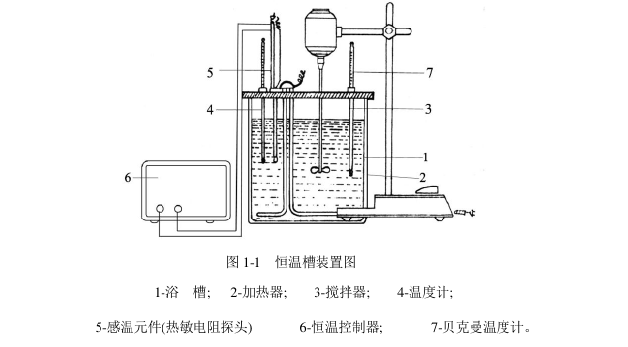
\includegraphics[width=.9\linewidth]{../img/1.png}
\end{center}

上图即是一恒温装置。它由浴槽、加热器、搅拌器、温度计、感温元件、恒温控制
器等组成,现分别介绍如下:

\begin{itemize}
\item 浴槽: 通常用的是 10dm\textsuperscript{3} 的圆柱形玻璃容器。槽内一般放蒸馏水,如恒温的温度超过了 100\textsuperscript{o}C可采用液体石腊和甘油。温度控制的范围不同,水浴槽中介质也不同,一般来说:
\begin{itemize}
\item -60\textsuperscript{o}C\(\sim\) 30\textsuperscript{o}C时使用乙醇或乙醇水溶液
\item 0\textsuperscript{o}C\(\sim\) 90\textsuperscript{o}时使用水
\item 80\textsuperscript{o}C\(\sim\) 160\textsuperscript{o}C时使用甘油或甘油水溶液
\item 70\textsuperscript{o}C\(\sim\) 200\textsuperscript{o}C时使用液体石蜡,硅油等
\end{itemize}
\item 加热器:常用的是电热器,我们用的电加热器把电阻丝放入环形的玻璃管中,根据浴槽的直径大小弯曲成圆环制成。它可以把加热丝放出的热量均匀地分布在圆形恒温槽的周围。电加热器由电子继电器进行自动调节,以实现恒温。电加热器的功率是根据恒温槽的容量、恒温控制的温度以及和环境的温差大小来决定的。最好能使加热和停止加热的时间各占一半。为了提高恒温的效果和精度,我们在恒温控制器和电加热器之间串接一只 1kV 的可调变压器, 其恒温槽的电路图设计如下:
\begin{center}
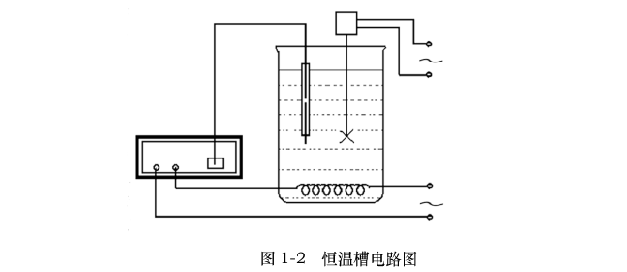
\includegraphics[width=.9\linewidth]{../img/2.png}
\end{center}实验开始时,由于室温距恒定温度的温差较大,为了尽快升温达到恒定温度,我们就把串接的输出电压调高一些,而待其温度逐渐接近恒温温度时,为了减少滞后现象,要把可调变压器的输出电压调低一点, 这样能较好地提高恒温槽控温的精度.

\item 搅拌器: 一般采用功率为 40W 的电动搅拌器,并将该电动搅拌器串联在一个可调变压器上用来调节搅拌的速度,使恒温槽各处的温度尽可能地相同。搅拌器安装的位置,桨叶的形状对搅拌效果都有很大的影响。为此搅拌桨叶应是螺旋桨式的或涡轮式的,且有适当片数, 直径和面积, 以使液体在恒温槽中循环, 保证恒温槽整体温度的均匀性.

\item 温度计:恒温槽中常以一支测量恒1/10\textsuperscript{o}C的温度计测量恒温槽的温度。用贝克曼温度计测量恒温槽的灵敏度, 所用的温度计在使用前都必须进行矫正和标化

\item 恒温控制器: 我们实验室采用的温控仪是 DTC-2AI 型有测温部件的控温仪。它采用稳定性能较好的热敏电阻作为感温元件,感温时间较短、使用方便、调速快、精度高并能进行遥控遥测。这个感温元件又因使用了特殊的烧结工艺,故只需要将此感温元件(探头)放在所需的控温部位,就能在控温的同时,从测温仪表上精确地反应出被控温部位的温度值。如图所示。
\begin{center}
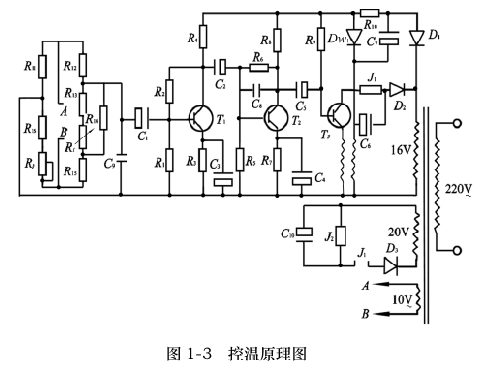
\includegraphics[width=.9\linewidth]{../img/3.png}
\end{center}
\end{itemize}




超级恒温水浴属于“通”“断”二端式控温,因此不可避免地存在着一定的滞后现象,
如温度的传递、感温元件(热敏探头或接触式温度计)继电器、电加热器等的滞后。所以恒温
槽控制的温度存在有一定的波动范围,而不是控制在某一固定不变的温度。其波动范围越小,
槽内各处的温度越均匀,恒温槽的灵敏度越高。灵敏度的高低是衡量恒温槽恒温优劣的主要
标志,它不仅与温控仪所选择的感温元件、继电器、接触式温度计等灵敏度有关,而且与搅
拌器的效率、加热器的功率、恒温槽的大小等因素有关。搅拌的效率越高,温度越易达到均
匀,恒温效果越好。加热器的功率用可调变压器进行调节,以保证在恒温槽达到所需的温度
后减小电加热的余热,减小温度过高或过低地偏离恒定温度的程度。此外,恒温槽装置内的
各个部件的布局对恒温槽的灵敏度也有一定的影响。一般布局原则是:加热器与搅拌器应放
得近一些,这样利于热量的传递。本论文通过对八组实验数据的处理,分析恒温槽在不同条
件下的灵敏度。

\part{实验部分}
\label{sec:orgf64cf7b}
\chapter{实验仪器与试剂}
\label{sec:orge2afea6}
\section{仪器}
\label{sec:orgada4166}
\begin{center}
\begin{tabular}{lr}
仪器 & 数目\\
\hline
商业恒温槽 & 1\\
电子温差仪及配套计算机 & 1\\
贝克曼温度计 & 1\\
继电器及相关导线等 & 1\\
循环冷却水设备 & 1\\
\end{tabular}
\end{center}


\chapter{实验步骤}
\label{sec:org2292a41}
\section{装配恒温槽}
\label{sec:orgeb21e7c}
调节接触温度计,连接线路,将温度设定为 35.00\textsuperscript{o}C。
\section{恒温槽灵敏度测量}
\label{sec:orgf78fd09}
\begin{enumerate}
\item 不通入冷却水
\label{sec:org61a0231}
\begin{enumerate}
\item 温度达到 35.00\textsuperscript{o}C 后,分别将调压器调节为 125V 和 200V 两个加热电压,等继电器不断地开关跳动表现恒温以后,然后用电子数字温差计测量温差\(\Delta\) T 与时间 t 的变化曲线: \(\Delta\) T(\textsuperscript{o}C)\(\sim\) t(sec)

\item 改变线路,使用仪器自身所带调温系统,用电子数字温差计测量温差\(\Delta\) T 与时间 t 的变化曲线: \(\Delta\) T(\textsuperscript{o}C)\(\sim\) t(sec)
\end{enumerate}
\item 通入冷却水
\label{sec:org3860e39}
\begin{enumerate}
\item 温度达到 35.00\textsuperscript{o}C 后, 通入冷却水, 分别将调压器调节为 125V 和 200V 两个加热电压,等继电器不断地开关跳动表现恒温以后,然后用电子数字温差计测量温差\(\Delta\) T 与时间 t 的变化曲线: \(\Delta\) T(\textsuperscript{o}C)\(\sim\) t(sec)

\item 改变线路,使用仪器自身所带调温系统,用电子数字温差计测量温差\(\Delta\) T 与时间 t 的变化曲线: \(\Delta\) T(\textsuperscript{o}C)\(\sim\) t(sec)
\end{enumerate}
\end{enumerate}
\chapter{实验数据及数据处理(见附件)}
\label{sec:org54f880c}
\chapter{结果分析与讨论}
\label{sec:org6eda7e4}
\section{实验结果}
\label{sec:org2ef71eb}
\begin{enumerate}
\item 灵敏度
\label{sec:orgddf91fe}
\begin{center}
\begin{tabular}{rll}
序号 & 恒温槽 & 灵敏度(\textsuperscript{o}C)\\
\hline
1 & DTC-2AI-200V-无冷却水 & \textpm{} 0.0130\\
2 & DTC-2AI-125V-无冷却水 & \textpm{} 0.0048\\
3 & DTC-2AI-200V-冷却水 & \textpm{} 0.0160\\
4 & DTC-2AI-125V-冷却水 & \textpm{} 0.0009\\
5 & 继电器-200V-无冷却水 & \textpm{} 0.0604\\
6 & 继电器-125V-无冷却水 & \textpm{} 0.0254\\
7 & 继电器-200V-冷却水 & \textpm{} 0.0712\\
8 & 继电器-125V-冷却水 & \textpm{} 0.0266\\
 &  & \\
\end{tabular}
\end{center}
\item 绘图
\label{sec:org57588aa}
\begin{enumerate}
\item DTC-2AI-200V-无冷却水
\label{sec:orgb031126}
\begin{center}
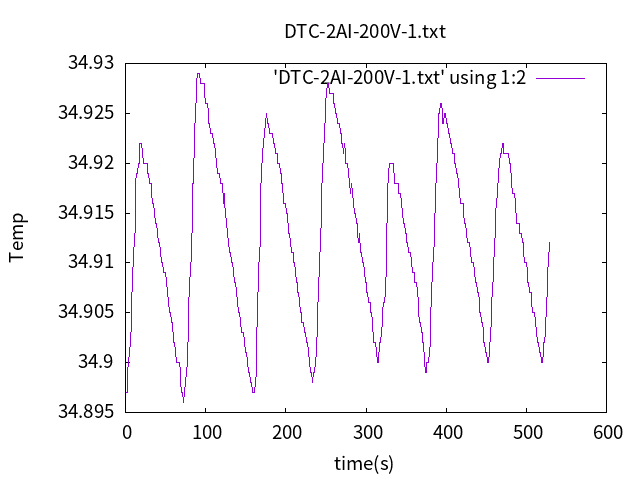
\includegraphics[width=.9\linewidth]{../img/DTC-2AI-200V-1.txt.png}
\end{center}
\item DTC-2AI-125V-无冷却水
\label{sec:org314e972}
\begin{center}
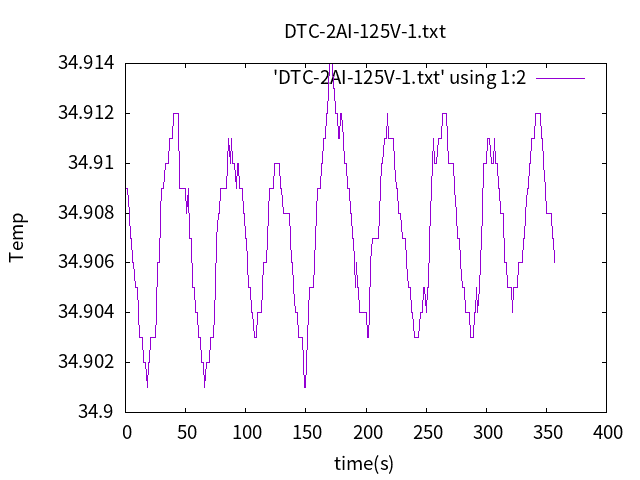
\includegraphics[width=.9\linewidth]{../img/DTC-2AI-125V-1.txt.png}
\end{center}
\item DTC-2AI-200V-冷却水
\label{sec:org24c962a}
\begin{center}
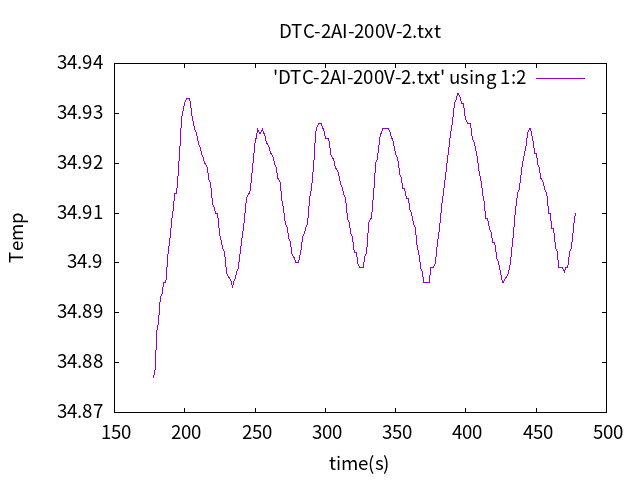
\includegraphics[width=.9\linewidth]{../img/DTC-2AI-200V-2.txt.png}
\end{center}
\item DTC-2AI-125V-冷却水
\label{sec:org33b5963}
\begin{center}
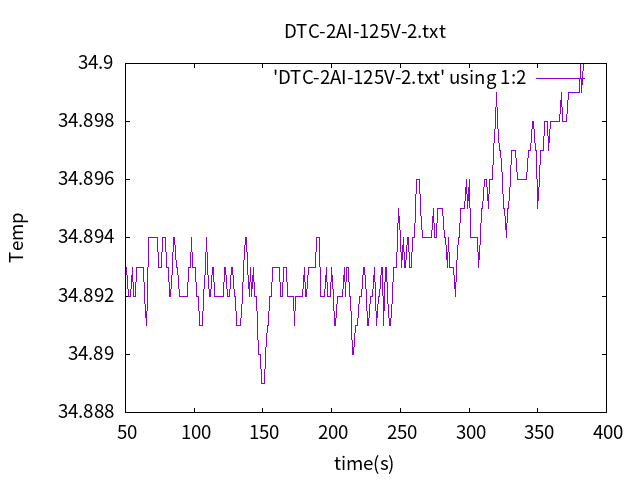
\includegraphics[width=.9\linewidth]{../img/DTC-2AI-125V-2.txt.png}
\end{center}
\item 继电器-200V-无冷却水
\label{sec:orgc049b05}
\begin{center}
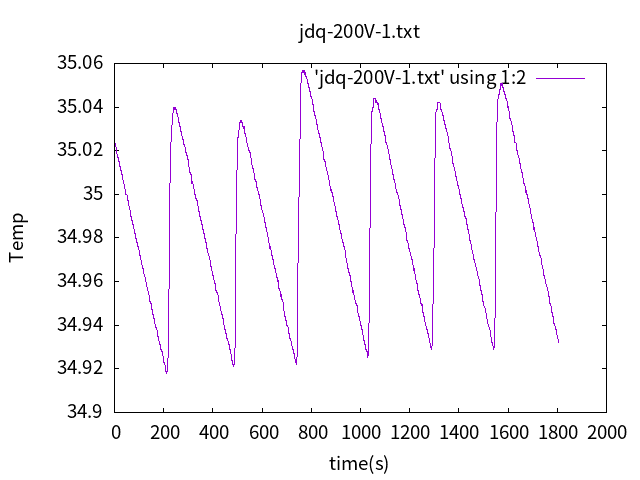
\includegraphics[width=.9\linewidth]{../img/jdq-200V-1.txt.png}
\end{center}
\item 继电器-125V-无冷却水
\label{sec:org9468556}
\begin{center}
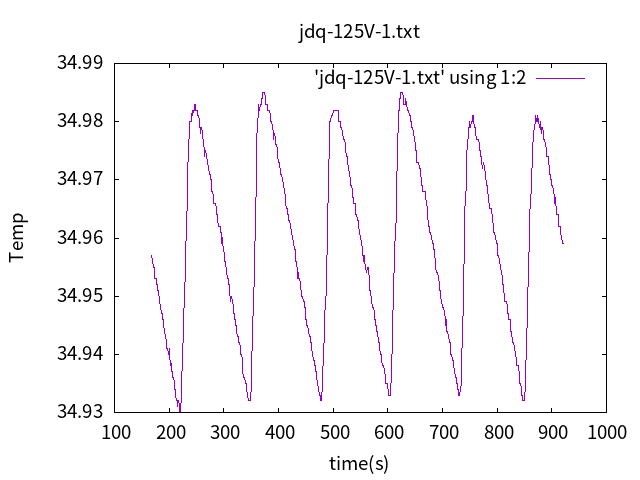
\includegraphics[width=.9\linewidth]{../img/jdq-125V-1.txt.png}
\end{center}
\item 继电器-200V-冷却水
\label{sec:org1f8513f}
\begin{center}
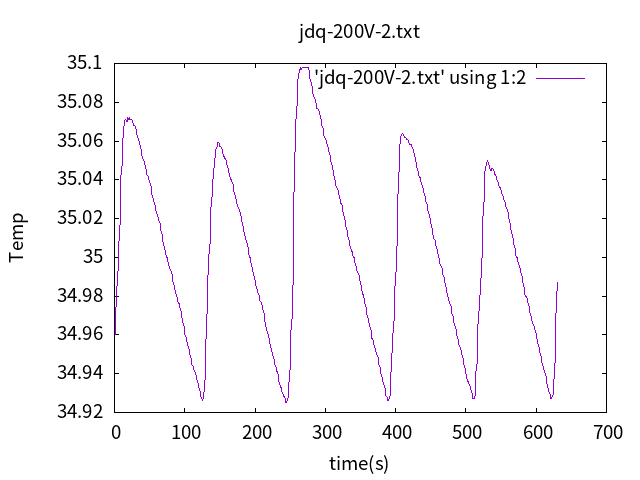
\includegraphics[width=.9\linewidth]{../img/jdq-200V-2.txt.png}
\end{center}
\item 继电器-125V-冷却水
\label{sec:orgb239e90}
\begin{center}
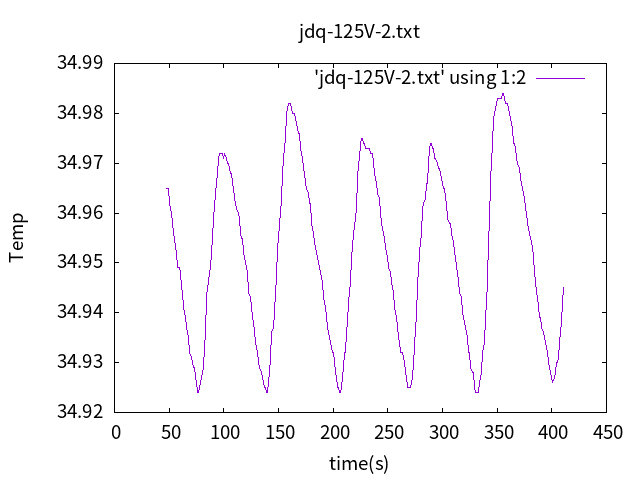
\includegraphics[width=.9\linewidth]{../img/jdq-125V-2.txt.png}
\end{center}
\end{enumerate}
\end{enumerate}
\section{实验讨论}
\label{sec:org0eedf25}
\begin{enumerate}
\item 比较1,3;2,4
\label{sec:org121e766}
同样是自动控温,区别在于 3,4 中通了循环水冷却,而冷却
水并不是该恒温槽的一部分。可以看出通了冷却水之后
的灵敏度以及波动的平稳性在不同电压下变化不一致。
所以可以得出结论, 冷却水对于自动控温器的影响不大
\item 比较5,7;6,8
\label{sec:orgc9bdf0a}
同样是继电器控温,区别依旧是有没有循环水。仔细比
较图像,有循环水的情况下温度上升段的速率变慢,而下降
段的速率变快,反应在图像上便是斜率的变小。这证实了在
机械控温情况下,冷却水的效果是加快散热,增长升温周期,
缩短降温半周期。加上循环水后温度波动范围也有所增加,
周期发生了一定程度的缩短, 可能与加热的速率(远)
大于冷却水降温速率有关
\item 比较2,1;4,3
\label{sec:orgbfa0f8c}
电压由 125V 增加到 200V,即加热功率上升,过快的加热速
率会导致体系偏离平衡的程度增加,不稳定程度也随之增加。
可以推断出温度波动范围会增大,这也被图像所证实。此外,
电压上升还导致了温度波动周期的增大,这应该是由于波动
范围的增大与温度改变(主要是降温)速度保持不变引起的。
\item 比较自动控温和机械控温
\label{sec:orgfd27cc5}
灵敏度的差距将在后面讨论,这里要说的自动控温下温度波
动周期远小于机械控温。波动周期显然也是恒温槽性能的重
要表征之一。对于使用恒温槽进行的具体实验来说,同样的
灵敏度情况下,小的周期使得起伏带来的系统误差更能够相
互补偿抵消。
\end{enumerate}

\section{结论}
\label{sec:org5b033c1}
\begin{enumerate}
\item 有无循环水的比较
\label{sec:org165b3e1}
机械控温下加入循环水会导致灵敏度的数值增大,
但对于自动控温的两种电压下,有无循环水对灵敏度的影响方向并不一致。
这也进一步暗示了两种控温原理上的不同——即自动控温周期可能并
不仅仅由恒定速率的升温和降温两个步骤组成。
\item 机械控温不同电压下比较
\label{sec:orgbd77b39}
机械控温下 200V 时的灵敏度大约为 125V 的两倍多。由此猜想
灵敏度与继电器电压之间可能存在着一些简单的正相关函数
关系,具体的函数可以通过热力学计算得出,进一步的实验
来验证(可以用来求散热系数之类的热力学参数!)。
\item 自动控温与机械控温比较
\label{sec:org9159f2c}
不论有无循环水,自动控温的灵敏度都远优于实验条件下的
机械控温, 而且就加热速度而言也相差无几, 这也说明了商业化的恒温槽控温能力的优异与稳定
性远不是我们简单的组装一下温度计和继电器能达到的。诚
然由上一条分析可以推断出,当机械控温的电压足够小的时
候可能达到所需的灵敏度, 但相应地也会损失加热的速度, 需要更先进的保温设备
\end{enumerate}
\section{误差分析}
\label{sec:orgec92fa8}
本实验应该算是一个半定量的实验,并没有通过最后的数据来
计算一些物理化学参数,只是通过对图像和数据的比较来得出一些
结论。从而总体上来说,试验中的误差对结论的影响相对较小。可
能的误差来源有以下两个方面。
\begin{enumerate}
\item 数据处理带来的误差
\label{sec:orga09bc36}
在对数据的处理过程中,采用不同的方法得出的灵敏度可能
会有很大的区别,这也是本实验误差的主要来源。取那一段
图像计算,如何确定最大值与最小值,如何处理数据的不利
波动等问题都会影响最后的结果。有些资料中是取一段图像,
利用平行线与图像相切进而求出灵敏度,但本次实验的数据每组的最大最小值
总体来说波动并不大, 所以并不需要那么做, 只要简单地找出其中的最大点最小点即可。


\item 系统误差
\label{sec:org39cd534}
继电器电压,冷却水温度,搅拌器速度等因素都可能导致系统误差,但对该实验来说并无大碍。
\end{enumerate}


\part{参考文献}
\label{sec:org780ca1d}
\begin{enumerate}
\item 中国科学技术大学物理化学实验室. 恒温槽的装配与性能测定
\item 周印希. 恒温槽灵敏度实验之简易精密温度控制装置的研制. 中国现代教育.装备 2010年第 23 期(总第 111 期)
\item 尹波.恒温槽调节与温度控制实验条件的探讨. 江西化工. 2008 年第 2 期
\item 物理化学讲义 科大物化实验组
\end{enumerate}


\part{附录: 数据处理过程}
\label{sec:orgffa929c}
\chapter{DTC-2AI}
\label{sec:orgcd14c6d}
\section{不通冷却水}
\label{sec:org5bbc6bf}
\begin{enumerate}
\item 200V
\label{sec:orgb6ab121}
\begin{center}
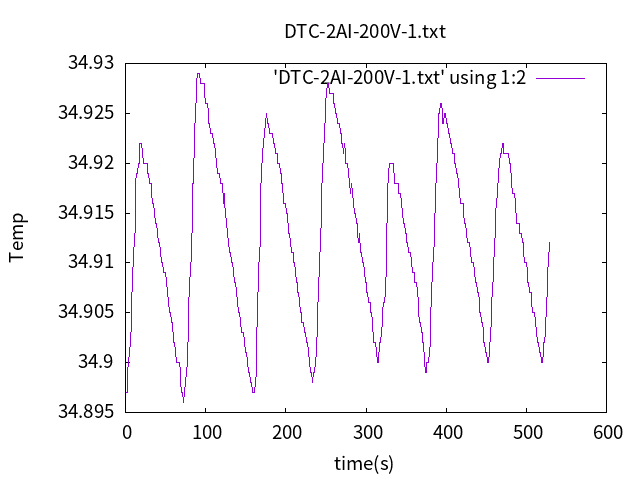
\includegraphics[width=.9\linewidth]{../img/DTC-2AI-200V-1.txt.png}
\end{center}

\begin{center}
\begin{tabular}{rrr}
序号 & 温度最大值(\textsuperscript{o}C) & 温度最小值(\textsuperscript{o}C)\\
\hline
1 & 34.922 & 34.896\\
2 & 34.929 & 34.897\\
3 & 34.925 & 34.898\\
4 & 34.928 & 34.900\\
5 & 34.920 & 34.899\\
6 & 34.926 & 34.900\\
7 & 34.922 & 34.900\\
平均 & 34.9246 & 34.8986\\
\end{tabular}
\end{center}

根据数据:
\begin{itemize}
\item 最大温度为: 34.9246°C
\item 最小温度为: 34.8986°C
\end{itemize}
所以恒温槽灵敏度为
\[
t=\pm\frac{t_{max}-t_{min}}{2}=\pm 0.0130^{o}C
\]


\item 125V
\label{sec:orge6d59e5}
\begin{center}
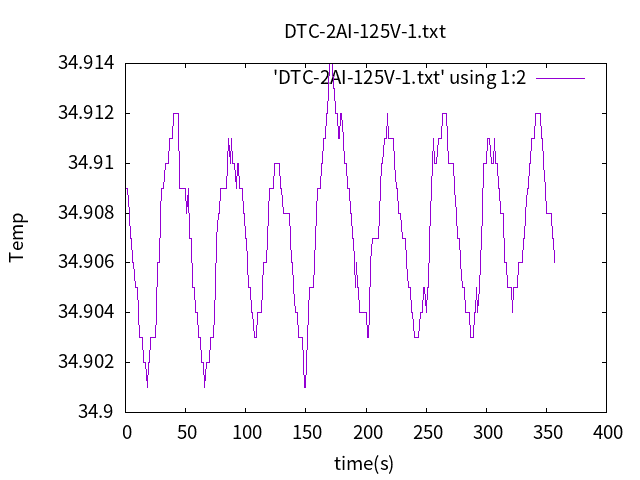
\includegraphics[width=.9\linewidth]{../img/DTC-2AI-125V-1.txt.png}
\end{center}
\begin{center}
\begin{tabular}{rrr}
序号 & 温度最大值(\textsuperscript{o}C) & 温度最小值(\textsuperscript{o}C)\\
\hline
1 & 34.912 & 34.901\\
2 & 34.911 & 34.901\\
3 & 34.910 & 34.903\\
4 & 34.914 & 34.901\\
5 & 34.912 & 34.903\\
6 & 34.912 & 34.903\\
7 & 34.911 & 34.903\\
8 & 34.912 & 34.903\\
平均 & 34.9118 & 34.9023\\
\end{tabular}
\end{center}

根据数据:
\begin{itemize}
\item 最大温度为: 34.9118°C
\item 最小温度为: 34.9023°C
\end{itemize}
所以恒温槽灵敏度为
\[
t=\pm\frac{t_{max}-t_{min}}{2}=\pm 0.0048^{o}C
\]
\end{enumerate}



\section{通冷却水}
\label{sec:orga1ed473}
\begin{enumerate}
\item 200V
\label{sec:org61c5db0}
\begin{center}
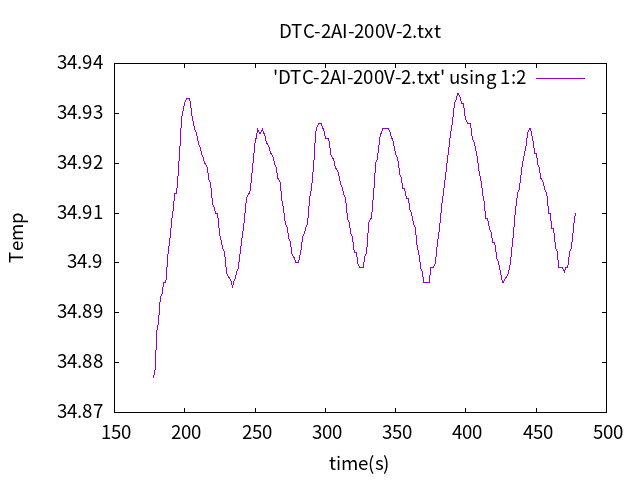
\includegraphics[width=.9\linewidth]{../img/DTC-2AI-200V-2.txt.png}
\end{center}
\begin{center}
\begin{tabular}{rrr}
序号 & 温度最大值(\textsuperscript{o}C) & 温度最小值(\textsuperscript{o}C)\\
\hline
1 & 34.933 & 34.895\\
2 & 34.927 & 34.900\\
3 & 34.928 & 34.899\\
4 & 34.927 & 34.896\\
5 & 34.934 & 34.896\\
6 & 34.927 & 34.898\\
平均 & 34.9293 & 34.8973\\
\end{tabular}
\end{center}

根据数据:
\begin{itemize}
\item 最大温度为: 34.9293°C
\item 最小温度为: 34.8973°C
\end{itemize}
所以恒温槽灵敏度为
\[
t=\pm\frac{t_{max}-t_{min}}{2}=\pm 0.0160^{o}C
\]



\item 125V
\label{sec:org3d3c800}
\begin{center}
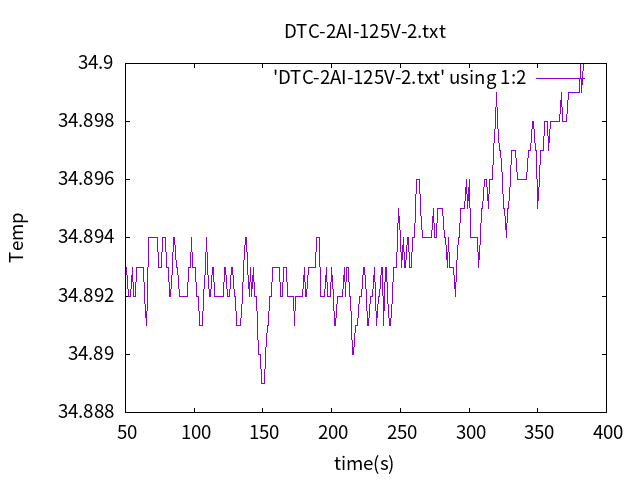
\includegraphics[width=.9\linewidth]{../img/DTC-2AI-125V-2.txt.png}
\end{center}
\begin{center}
\begin{tabular}{rrr}
序号 & 温度最大值(\textsuperscript{o}C) & 温度最小值(\textsuperscript{o}C)\\
\hline
1 & 34.894 & 34.893\\
2 & 34.894 & 34.892\\
3 & 34.894 & 34.892\\
4 & 34.894 & 34.891\\
5 & 34.894 & 34.892\\
6 & 34.893 & 34.892\\
平均 & 34.8938 & 34.8920\\
\end{tabular}
\end{center}

\begin{itemize}
\item 注: 图中250s后的数据被废弃掉了, 因为此时冷却水的流速发生了改变
\end{itemize}

根据数据:
\begin{itemize}
\item 最大温度为: 34.8938°C
\item 最小温度为: 34.8920°C
\end{itemize}
所以恒温槽灵敏度为
\[
t=\pm\frac{t_{max}-t_{min}}{2}=\pm 0.0009^{o}C
\]
\end{enumerate}


\chapter{继电器}
\label{sec:orgef788d7}
\section{不通冷却水}
\label{sec:org2348d97}
\begin{enumerate}
\item 200V
\label{sec:org335b3f0}
\begin{center}
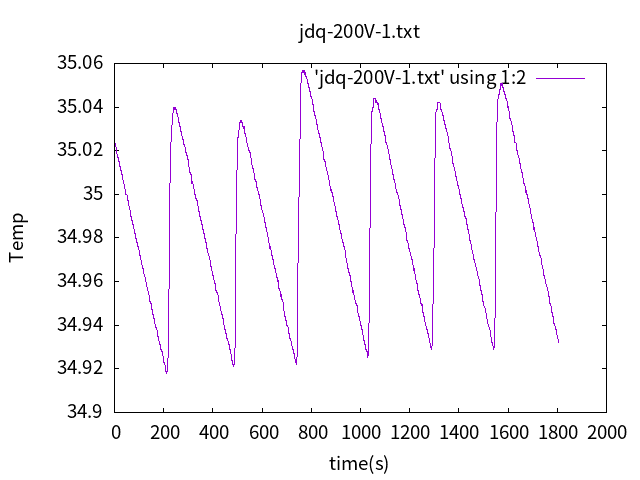
\includegraphics[width=.9\linewidth]{../img/jdq-200V-1.txt.png}
\end{center}
\begin{center}
\begin{tabular}{rrr}
序号 & 温度最大值(\textsuperscript{o}C) & 温度最小值(\textsuperscript{o}C)\\
\hline
1 & 35.040 & 34.918\\
2 & 35.034 & 34.921\\
3 & 35.057 & 34.922\\
4 & 35.044 & 34.925\\
5 & 35.042 & 34.929\\
6 & 35.051 & 34.929\\
平均 & 35.0447 & 34.9240\\
\end{tabular}
\end{center}

根据数据:
\begin{itemize}
\item 最大温度为: 35.0447°C
\item 最小温度为: 34.9240°C
\end{itemize}
所以恒温槽灵敏度为
\[
t=\pm\frac{t_{max}-t_{min}}{2}=\pm 0.0604^{o}C
\]


\item 125V
\label{sec:orgc92f4e1}
\begin{center}
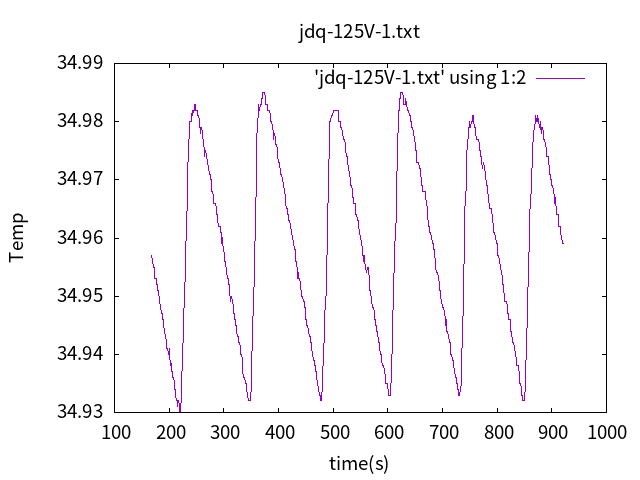
\includegraphics[width=.9\linewidth]{../img/jdq-125V-1.txt.png}
\end{center}
\begin{center}
\begin{tabular}{rrr}
序号 & 温度最大值(\textsuperscript{o}C) & 温度最小值(\textsuperscript{o}C)\\
\hline
1 & 34.983 & 34.930\\
2 & 34.985 & 34.932\\
3 & 34.982 & 34.932\\
4 & 34.985 & 34.933\\
5 & 34.981 & 34.933\\
6 & 34.981 & 34.932\\
平均 & 34.9828 & 34.9320\\
\end{tabular}
\end{center}

根据数据:
\begin{itemize}
\item 最大温度为: 34.9828°C
\item 最小温度为: 34.9320°C
\end{itemize}
所以恒温槽灵敏度为
\[
t=\pm\frac{t_{max}-t_{min}}{2}=\pm 0.0254^{o}C
\]
\end{enumerate}


\section{通冷却水}
\label{sec:org4fcb6c5}
\begin{enumerate}
\item 200V
\label{sec:orga394915}
\begin{center}
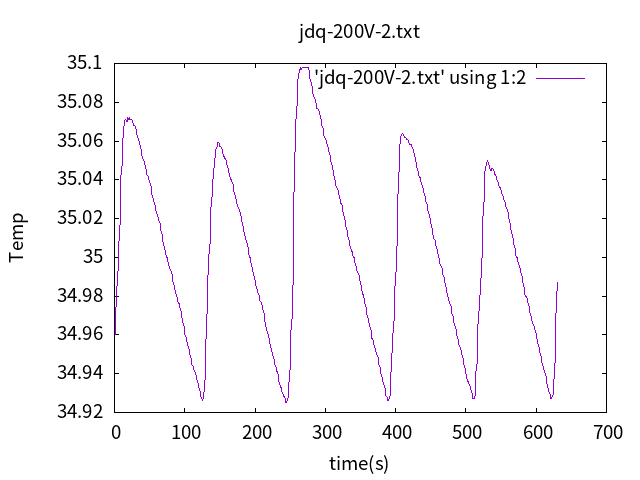
\includegraphics[width=.9\linewidth]{../img/jdq-200V-2.txt.png}
\end{center}
\begin{center}
\begin{tabular}{rrr}
序号 & 温度最大值(\textsuperscript{o}C) & 温度最小值(\textsuperscript{o}C)\\
\hline
1 & 35.072 & 34.926\\
2 & 35.059 & 34.925\\
3 & 35.098 & 34.926\\
4 & 35.064 & 34.927\\
5 & 35.050 & 34.927\\
平均 & 35.0686 & 34.9262\\
\end{tabular}
\end{center}

根据数据:
\begin{itemize}
\item 最大温度为: 35.0686°C
\item 最小温度为: 34.9262°C
\end{itemize}
所以恒温槽灵敏度为
\[
t=\pm\frac{t_{max}-t_{min}}{2}=\pm 0.0712^{o}C
\]


\item 125V
\label{sec:org747e9c3}
\begin{center}
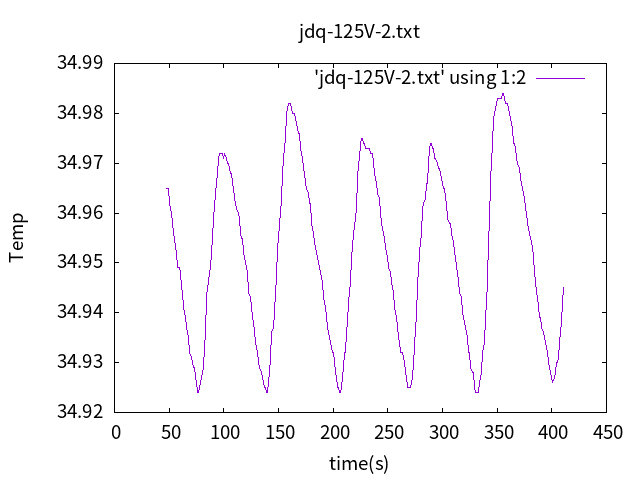
\includegraphics[width=.9\linewidth]{../img/jdq-125V-2.txt.png}
\end{center}
\begin{center}
\begin{tabular}{rrr}
序号 & 温度最大值(\textsuperscript{o}C) & 温度最小值(\textsuperscript{o}C)\\
\hline
1 & 34.972 & 34.924\\
2 & 34.982 & 34.924\\
3 & 34.975 & 34.924\\
4 & 34.974 & 34.925\\
5 & 34.984 & 34.924\\
平均 & 34.9774 & 34.9242\\
\end{tabular}
\end{center}

根据数据:
\begin{itemize}
\item 最大温度为: 34.9774°C
\item 最小温度为: 34.9242°C
\end{itemize}
所以恒温槽灵敏度为
\[
t=\pm\frac{t_{max}-t_{min}}{2}=\pm 0.0266^{o}C
\]
\end{enumerate}
\end{document}
